\chapter{Ellinghamdiagrammen en metallurgie}\label{ch:b2:ellingham}

Een hoogoven zet rood gesteente om in vloeibaar ijzer met cokes en hete lucht, met
een tempo van duizenden ton per dag. Geen enkele oven van die soort zal ooit
aluminium, magnesium of titaan maken, hoewel koolstof voor die metalen even goedkoop is.
De meeste metalen worden in de bodem als oxiden gevonden, en een metaal winnen betekent
er de zuurstof uit wegnemen: welke reductoren dat kunnen, en bij welke
temperatuur, is een kwestie van standaardgibbsenergieën. In 1944 zette Harold
Ellingham ze allemaal in één diagram, als functie van de temperatuur, telkens voor één mol
dizuurstof. Het diagram toont in één oogopslag welk metaal welk oxide reduceert,
waarom koolstof bij hoge temperatuur wint, en waarom sommige metalen door
elektrolyse gemaakt moeten worden.

\begin{recall}
\Cref{ch:b2:reaction-free-energy}: $\Delta_r G^\circ = \Delta_r H^\circ -
T\Delta_r S^\circ$ en de \omterm{def:b2:reaction-free-energy:ellingham-approximation}{benadering van Ellingham} (rechte lijnen in $T$,
faseovergangen uitgezonderd). \Cref{ch:b2:equilibrium-shifts}: $K^\circ$ uit
$\Delta_r G^\circ$, \omterm{def:b2:equilibrium-shifts:variance}{variantie}, het einde van een evenwicht wanneer een fase
verdwijnt. Het deel van jaar~1: oxidatiegetallen, redoxkoppels, basische en
zure oxiden. Het schoolboek: ertsen.
\end{recall}

\begin{omfigure}
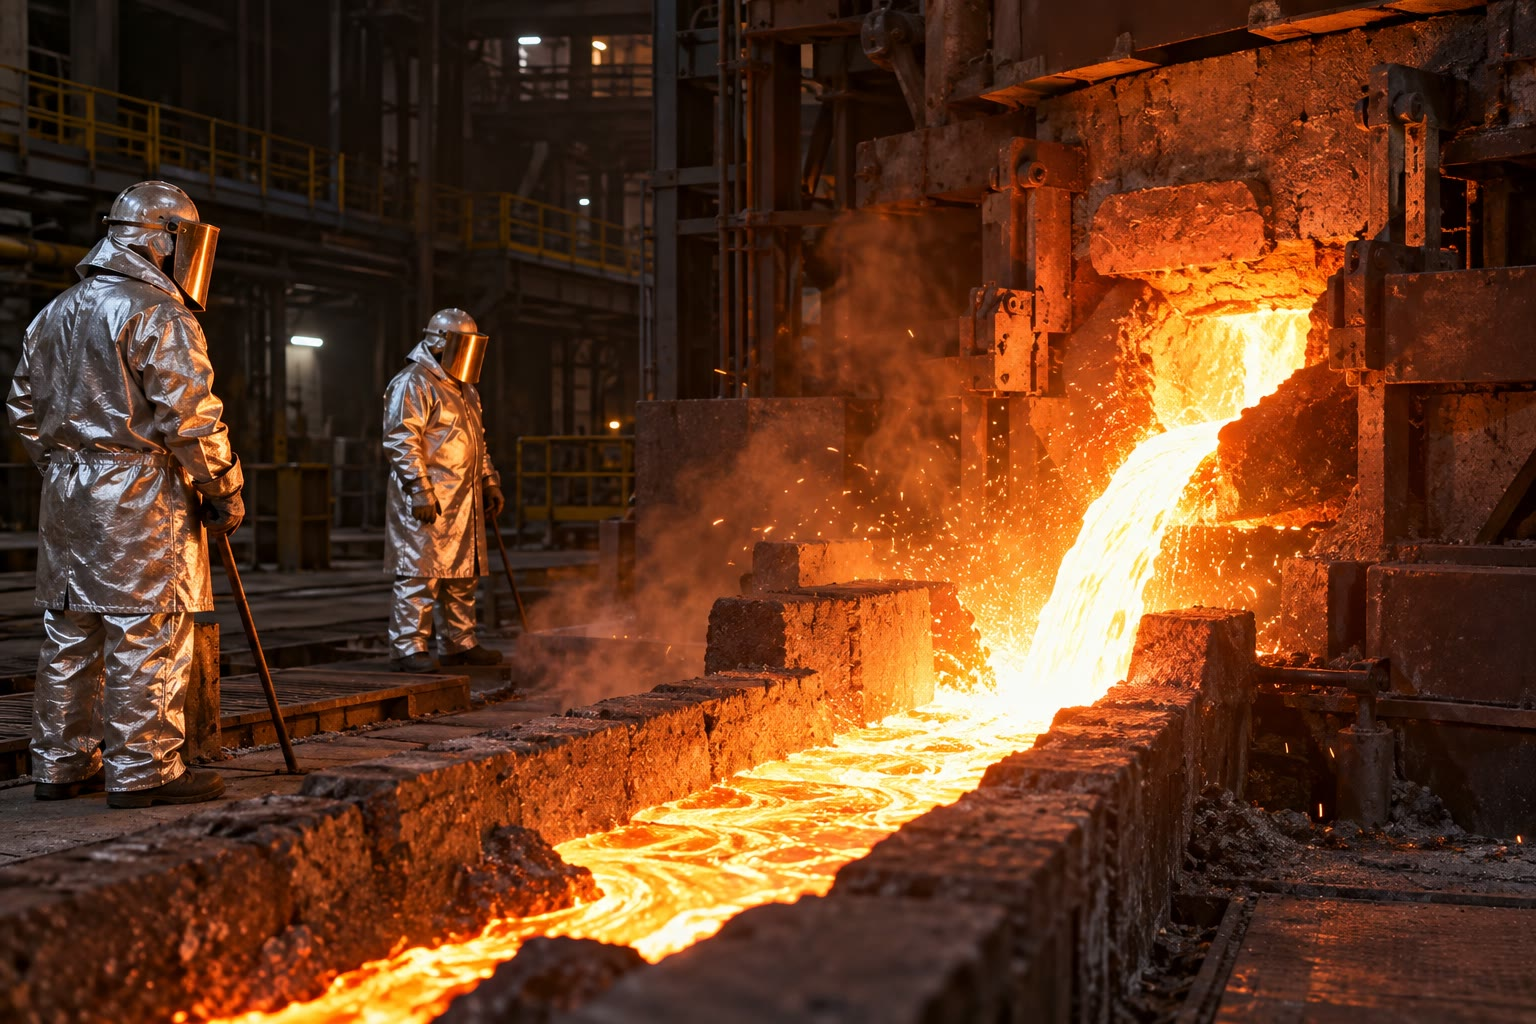
\includegraphics[width=0.62\linewidth]{images/book3/ai/b2-06-blast-furnace.jpg}

{\small Het aftappen van een hoogoven: vloeibaar ijzer stroomt door een vuurvaste goot,
in het oog gehouden door arbeiders in hittewerende pakken. De temperatuur en het gas
in de oven zijn die waarbij koolstofmonoxide de zuurstof kan wegnemen
uit ijzeroxide.}
\end{omfigure}

\section{Het ellinghamdiagram}

Om de affiniteit van verschillende metalen voor zuurstof te vergelijken, worden de reacties
zo geschreven dat ze allemaal dezelfde hoeveelheid van het gemeenschappelijke reagens verbruiken.

\begin{definition}[Ellinghamdiagram]\label{def:b2:ellingham:diagram}
Het \emph{ellinghamdiagram}\index{ellinghamdiagram} van een familie oxiden
is de grafiek, als functie van de temperatuur, van de standaardgibbsenergieën van hun
vormingsreacties, geschreven voor één mol dizuurstof,
\[
  \tfrac{2x}{y}\,\mathrm M + \ce{O2} \longrightarrow \tfrac{2}{y}\,\mathrm{M}_x\mathrm O_y ,
  \qquad \Delta_r G^\circ(T) \ \text{per mol } \ce{O2} .
\]
\end{definition}

Bijvoorbeeld \ce{2Zn + O2 -> 2ZnO}, \ce{4/3Al + O2 -> 2/3Al2O3}, \ce{2C + O2 ->
2CO}. De ordinaat staat in \unit{kJ} per mol \ce{O2}, steeds negatief voor de
metalen van het diagram.

\begin{proposition}[Rechte lijnen]\label{prop:b2:ellingham:line}
In de \omterm{def:b2:reaction-free-energy:ellingham-approximation}{benadering van Ellingham} is elke lijn recht, met helling $-\Delta_r
S^\circ$. Voor een metaal en zijn oxide, beide gecondenseerd, ligt $\Delta_r S^\circ$
dicht bij min de entropie van de verbruikte mol dizuurstof, ongeveer
$-\qty{200}{J/(K.mol)}$: de lijnen stijgen met de temperatuur, alle met bijna
dezelfde helling.
\end{proposition}

\begin{proof}
$\Delta_r G^\circ = \Delta_r H^\circ - T\Delta_r S^\circ$ met constante $\Delta_r
H^\circ$, $\Delta_r S^\circ$. De molaire entropieën van vaste stoffen bedragen tientallen
\unit{J/(K.mol)} en vallen grotendeels weg tussen metaal en oxide, terwijl er één mol
gas verbruikt wordt, met entropie $S^\circ(\ce{O2}) = \qty{205}{J/(K.mol)}$. Voor zink:
$2(43.65) - 2(41.63) - 205.15 = \qty{-201.1}{J/(K.mol)}$.
% ledger: s0:ZnO_cr, s0:Zn_cr, s0:O2_g
\end{proof}

\begin{proposition}[Knikken in de lijnen]\label{prop:b2:ellingham:break}
Bij de temperatuur waarbij het metaal smelt of kookt, verandert de lijn van helling:
haar helling neemt toe met $\nu\,\Delta_{\text{trs}}S$, waarin $\nu$ de hoeveelheid
metaal in de reactie is en $\Delta_{\text{trs}}S = \Delta_{\text{trs}}H/T_{\text{trs}}$.
Een faseovergang van het oxide verkleint de helling daarentegen.
\end{proposition}

\begin{proof}
Boven de overgang reageert het metaal vanuit zijn nieuwe fase, waarvan de entropie
$\Delta_{\text{trs}}S$ hoger is: $\Delta_r S^\circ$ neemt af met $\nu\,\Delta_{\text{trs}}S$
en de helling $-\Delta_r S^\circ$ neemt evenveel toe. $\Delta_r G^\circ$
zelf is continu, omdat bij $T_{\text{trs}}$ beide fasen dezelfde
\omterm{def:b2:chemical-potential:chemical-potential}{chemische potentiaal} hebben. Voor het oxide geldt het omgekeerde teken.
\end{proof}

Smelten verandert de helling een beetje; koken, dat een gecondenseerde beginstof
in een gas verandert, verandert haar sterk. Zink kookt bij \qty{1180}{K}: boven die
temperatuur verbruikt de vorming van zinkoxide drie mol gas per twee mol
oxide, en haar lijn klimt steil. Hetzelfde gebeurt met magnesium boven zijn
kookpunt.

\begin{omfigure}
\begin{tikzpicture}[lab/.style={anchor=west, font=\scriptsize, inner sep=1pt}]
\begin{axis}[omellingham,
  width=0.84\linewidth, height=11cm, xmin=300, xmax=2100, ymin=-1250, ymax=0,
  clip mode=individual,
  xlabel={$T$ (K)}, ylabel={$\Delta_r G^\circ$ (\unit{kJ} per mol \ce{O2})},
  xtick={300,500,700,900,1100,1300,1500,1700,1900,2100},
  x tick label style={rotate=45, anchor=north east, font=\scriptsize}]
\addplot[black!60, thick] table[x=T, y=G] {figdata/out/bachelor-2-ellingham-a-HgO.dat};
\addplot[omProp, thick] table[x=T, y=G] {figdata/out/bachelor-2-ellingham-a-Cu2O.dat};
\addplot[omDef, thick] table[x=T, y=G] {figdata/out/bachelor-2-ellingham-a-FeO.dat};
\addplot[omExo, very thick] table[x=T, y=G] {figdata/out/bachelor-2-ellingham-a-ZnO.dat};
\addplot[black!60, thick] table[x=T, y=G] {figdata/out/bachelor-2-ellingham-a-Cr2O3.dat};
\addplot[omProp, thick] table[x=T, y=G] {figdata/out/bachelor-2-ellingham-a-TiO2.dat};
\addplot[omDef, thick] table[x=T, y=G] {figdata/out/bachelor-2-ellingham-a-Al2O3.dat};
\addplot[black!60, thick] table[x=T, y=G] {figdata/out/bachelor-2-ellingham-a-MgO.dat};
\addplot[omProp, thick] table[x=T, y=G] {figdata/out/bachelor-2-ellingham-a-CaO.dat};
\addplot[omThm, very thick] table[x=T, y=G] {figdata/out/bachelor-2-ellingham-a-C-CO.dat};
\addplot[omThm, thick, dashed] table[x=T, y=G] {figdata/out/bachelor-2-ellingham-a-C-CO2.dat};
\addplot[omThm, thick, dotted] table[x=T, y=G] {figdata/out/bachelor-2-ellingham-a-CO-CO2.dat};
\addplot[omDef, thick, dashed] table[x=T, y=G] {figdata/out/bachelor-2-ellingham-a-H2-H2O.dat};
% labels: inside for the two short lines, at the right end for the others
\node[font=\scriptsize, black!70, anchor=south] at (axis cs:400,-60) {\ce{HgO}};
\node[font=\scriptsize, omProp, anchor=south] at (axis cs:1100,-150) {\ce{Cu2O}};
\draw[omExo, thin] (axis cs:2100,-69) -- (axis cs:2150,-60) node[lab, text=omExo] {\ce{ZnO}};
\draw[omThm, thin] (axis cs:2100,-204) -- (axis cs:2150,-185) node[lab, text=omThm] {\ce{CO}/\ce{CO2}};
\draw[omDef, thin] (axis cs:2100,-259) -- (axis cs:2150,-235) node[lab, text=omDef] {\ce{H2}/\ce{H2O}};
\draw[omDef, thin] (axis cs:2100,-286) -- (axis cs:2150,-285) node[lab, text=omDef] {\ce{FeO}};
\draw[black!70, thin] (axis cs:2100,-393) -- (axis cs:2150,-365) node[lab, text=black!70] {\ce{Cr2O3}};
\draw[omThm, thin] (axis cs:2100,-396) -- (axis cs:2150,-415) node[lab, text=omThm] {\ce{C}/\ce{CO2}};
\draw[omProp, thin] (axis cs:2100,-567) -- (axis cs:2150,-540) node[lab, text=omProp] {\ce{TiO2}};
\draw[omThm, thin] (axis cs:2100,-589) -- (axis cs:2150,-590) node[lab, text=omThm] {\ce{C}/\ce{CO}};
\draw[black!70, thin] (axis cs:2100,-600) -- (axis cs:2150,-640) node[lab, text=black!70] {\ce{MgO}};
\draw[omDef, thin] (axis cs:2100,-668) -- (axis cs:2150,-690) node[lab, text=omDef] {\ce{Al2O3}};
\draw[omProp, thin] (axis cs:2100,-765) -- (axis cs:2150,-765) node[lab, text=omProp] {\ce{CaO}};
\end{axis}
\end{tikzpicture}

{\small Het \omterm{def:b2:ellingham:diagram}{ellinghamdiagram}: standaardvormingsgibbsenergie van oxiden
per mol \ce{O2}, als functie van de temperatuur, uit getabelleerde gibbsenergieën. Hoe
lager een lijn, hoe stabieler het oxide en hoe sterker reducerend het metaal.
Elke metaallijn draagt de naam van haar oxide; \ce{C}/\ce{CO} is \ce{2C + O2 -> 2CO},
\ce{C}/\ce{CO2} is \ce{C + O2 -> CO2}, \ce{CO}/\ce{CO2} is \ce{2CO + O2 -> 2CO2}
en \ce{H2}/\ce{H2O} is \ce{2H2 + O2 -> 2H2O}, met water als gas.}
% ledger: janafG:Cu2O.300, janafG:FeO.300, janafG:Cr2O3.300, janafG:TiO2.500, janafG:Al2O3.300, janafG:MgO.300, janafG:CaO.300, janafG:CO.300, janafG:CO2.300, janafG:H2O.300, dfh:ZnO_cr, dfh:HgO_cr, s0:HgO_cr, s0:Hg_l, s0:Hg_g, dfh:Hg_g (all temperatures in figdata/bachelor-2/ellingham.py)
\end{omfigure}

\section{Het diagram lezen}

\begin{definition}[Evenwichtszuurstofdruk]\label{def:b2:ellingham:oxygen-pressure}
De \emph{evenwichtszuurstofdruk}\index{evenwichtszuurstofdruk} van een
paar metaal–oxide bij temperatuur $T$ is de druk van dizuurstof waarbij metaal
en oxide in evenwicht naast elkaar bestaan: $RT\ln(p_{\ce{O2}}/p^\circ) = \Delta_r
G^\circ(T)$ voor de reactie geschreven per mol \ce{O2}.
\end{definition}

\begin{theorem}[Gebieden van het metaal en van het oxide]\label{thm:b2:ellingham:domains}
In een atmosfeer met zuurstofdruk $p_{\ce{O2}}$ bij temperatuur $T$ wordt het
metaal geoxideerd als $RT\ln(p_{\ce{O2}}/p^\circ) > \Delta_r G^\circ(T)$, en wordt het
oxide gereduceerd tot het metaal als $RT\ln(p_{\ce{O2}}/p^\circ) < \Delta_r
G^\circ(T)$. In het diagram is het oxide stabiel boven zijn lijn, het metaal
eronder.
\end{theorem}

\begin{proof}
Met gecondenseerd metaal en oxide met activiteit 1 is $Q = p^\circ/p_{\ce{O2}}$ en
$\Delta_r G = \Delta_r G^\circ + RT\ln Q = \Delta_r G^\circ - RT\ln(p_{\ce{O2}}/
p^\circ)$. De oxidatie verloopt voorwaarts wanneer $\Delta_r G < 0$.
\end{proof}

Onder lucht ($p_{\ce{O2}} = \qty{0.21}{bar}$; $RT\ln 0.21$ is \qty{-4}{kJ/mol}
bij kamertemperatuur en \qty{-13}{kJ/mol} bij \qty{1000}{K}, op deze
schaal bijna nul) wordt elk metaal van het diagram waarvan de lijn
onder de as ligt, geoxideerd: bij kamertemperatuur allemaal, zelfs koper.
Alleen de oxiden bovenaan (zilver, kwik) ontleden bij matige
verhitting.

\begin{example}[Het oxide van kwik]\label{ex:b2:ellingham:hgo}
Voor \ce{2Hg + O2 -> 2HgO} geven de CODATA-sleutelwaarden $\Delta_r H^\circ =
\qty{-181.6}{kJ/mol}$ met vloeibaar kwik; boven het kookpunt van kwik
is het metaal een gas en is $\Delta_r H^\circ = \qty{-304.3}{kJ/mol}$, $\Delta_r
S^\circ = \qty{-414.6}{J/(K.mol)}$. De lijn snijdt nul bij
$T = 304.3/0.4146 \approx \qty{734}{K}$: verhit boven die temperatuur in lucht,
of onder \qty{1}{bar} zuurstof, geeft rood kwikoxide zijn zuurstof af ---
zo werd zuurstof in 1774 voor het eerst geïsoleerd.
% ledger: dfh:HgO_cr, s0:HgO_cr, s0:Hg_l, s0:Hg_g, dfh:Hg_g, s0:O2_g (computed in figdata/bachelor-2/ellingham.py)
\end{example}

\begin{proposition}[Welk metaal welk oxide reduceert]\label{prop:b2:ellingham:reduction}
Bij een gegeven temperatuur reduceert een metaal M onder standaardomstandigheden het
oxide van een metaal N wanneer de lijn van M onder die van N ligt. De
\omterm{def:b2:reaction-free-energy:reaction-gibbs}{standaardreactie-gibbsenergie} van de reductie, per mol overgedragen \ce{O2}, is het
verschil van de twee ordinaten.
\end{proposition}

\begin{proof}
De reductie is de vorming van het oxide van M min die van het oxide van N, beide per
mol \ce{O2}: $\Delta_r G^\circ = \Delta_r G^\circ_{\mathrm M} - \Delta_r
G^\circ_{\mathrm N}$, negatief wanneer de lijn van M lager ligt.
\end{proof}

\begin{method}[Een ellinghamdiagram lezen]\label{met:b2:ellingham:read-ellingham}
\begin{enumerate}
  \item Zoek de twee lijnen bij de gewenste temperatuur. De onderste is
        het stabielere oxide; zijn metaal reduceert het andere oxide.
  \item De verticale afstand is $\Delta_r G^\circ$ per mol \ce{O2}: een afstand van
        \qty{100}{kJ} of meer betekent een praktisch volledige reductie.
  \item Waar twee lijnen elkaar snijden, keert de reductie van richting om: lees de
        snijtemperatuur af.
  \item Let op de knikken: een metaal dat binnen het interval kookt, vertrekt als
        damp, die kan worden afgedestilleerd --- of die bij afkoeling opnieuw oxideert.
\end{enumerate}
\end{method}

\begin{definition}[Aluminothermische reductie]\label{def:b2:ellingham:aluminothermy}
Een \emph{aluminothermische reductie}\index{aluminothermische reductie} is de
reductie van een metaaloxide door aluminiumpoeder, mogelijk voor elk oxide waarvan de
lijn boven die van aluminiumoxide ligt, en zo \omterm{def:b2:reaction-enthalpy:exothermic}{exotherm} dat het mengsel smelt:
\ce{Fe2O3 + 2Al -> Al2O3 + 2Fe} (thermiet) last spoorstaven; \ce{Cr2O3 + 2Al ->
Al2O3 + 2Cr} levert koolstofvrij chroom.
\end{definition}

\begin{omfigure}
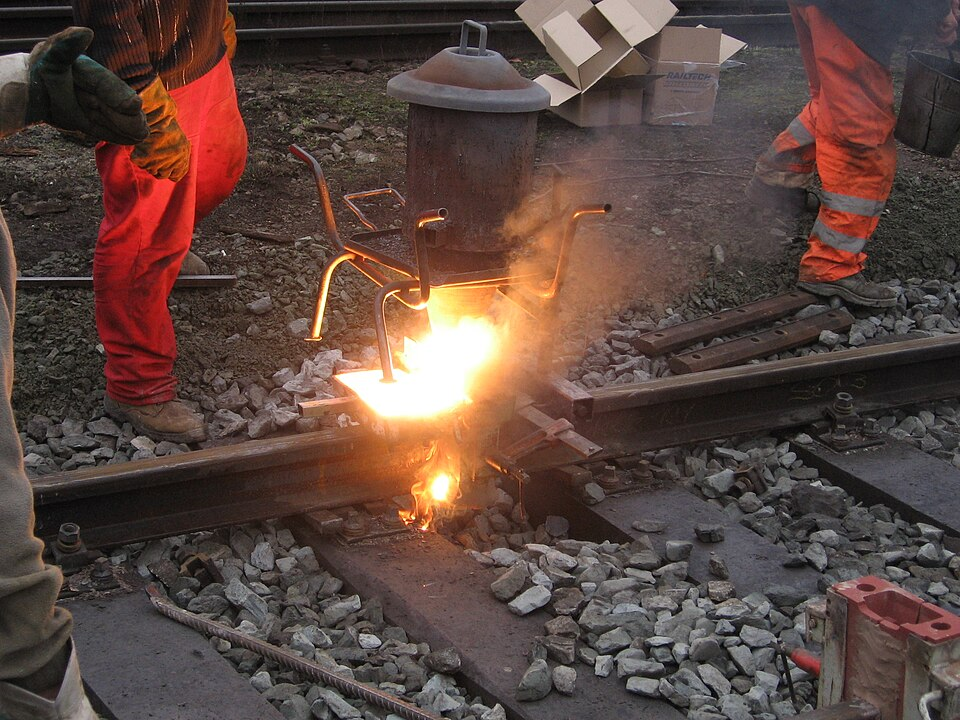
\includegraphics[width=0.5\linewidth]{images/book3/thermite.jpg}

{\small Thermietlassen van een spoorstaaf: de reactie van ijzeroxide met aluminium
in de kroes boven de voeg levert vloeibaar ijzer, dat in de
gietvorm tussen de twee spoorstaafuiteinden loopt. (Foto: PetrS., CC BY-SA 3.0, Wikimedia
Commons.)}
\end{omfigure}

\section{Koolstof en koolstofmonoxide}

Drie lijnen hebben met koolstof te maken:
\begin{itemize}
  \item \ce{C + O2 -> CO2}: één mol gas geeft er één, $\Delta_r S^\circ
        \approx 0$, een bijna horizontale lijn rond \qty{-395}{kJ};
  \item \ce{2C + O2 -> 2CO}: één mol gas geeft er twee, $\Delta_r S^\circ
        \approx \qty{+180}{J/(K.mol)}$, een lijn die met de temperatuur \emph{daalt};
  \item \ce{2CO + O2 -> 2CO2}: drie mol gas geven er twee, een stijgende lijn.
\end{itemize}

\begin{proposition}[Koolstof reduceert heet bijna alles]\label{prop:b2:ellingham:carbon}
De lijn van \ce{2C + O2 -> 2CO} daalt met de temperatuur en snijdt de
lijnen van de meeste metaaloxiden: boven de snijtemperatuur reduceert koolstof het
oxide, met vorming van koolstofmonoxide. Het snijpunt voor ijzer(II)oxide ligt rond
\qty{1040}{K}, voor zinkoxide rond \qty{1220}{K}; voor titaandioxide en magnesiumoxide ligt het
rond of boven \qty{2000}{K}, voor aluminiumoxide nog hoger, waar de metalen
met koolstof carbiden vormen of opnieuw oxideren terwijl het gas afkoelt.
\end{proposition}

\begin{proof}
De helling $-\Delta_r S^\circ$ van de koolstoflijn is negatief ($\Delta\nu_{\text{gas}}
= +1$), die van de oxidelijnen positief: ze snijden elkaar één keer. De temperaturen
zijn afgelezen op de berekende lijnen.
% ledger: janafG:CO.900, janafG:CO.1100, janafG:FeO.900, janafG:FeO.1100 (crossings computed in figdata/bachelor-2/ellingham.py)
\end{proof}

\begin{definition}[Boudouardevenwicht]\label{def:b2:ellingham:boudouard}
Het \emph{boudouardevenwicht}\index{boudouardevenwicht} is \ce{C(s) + CO2(g) <=> 2CO(g)},
\omterm{def:b2:reaction-enthalpy:exothermic}{endotherm}, tussen koolstof en de twee oxiden van koolstof.
\end{definition}

\begin{proposition}[Samenstelling van het gas boven koolstof]\label{prop:b2:ellingham:boudouard}
Het systeem koolstof + \ce{CO} + \ce{CO2} heeft \omterm{def:b2:equilibrium-shifts:variance}{variantie} 2: bij gegeven $T$ en totale
druk $p$ ligt de molfractie $x$ van koolstofmonoxide vast door $x^2/(1 - x)
= K^\circ(T)\,p^\circ/p$. Bij \qty{1}{bar} is het gas bijna zuiver \ce{CO2}
onder \qty{700}{K} en bijna zuiver \ce{CO} boven \qty{1200}{K}; het snijpunt van
de drie koolstoflijnen, rond \qty{975}{K}, is de plaats waar $K^\circ = 1$.
\end{proposition}

\begin{proof}
Drie deeltjes, één reactie, twee fasen: $v = 3 - 1 + 2 - 2 = 2$. Met $p_{\ce{CO}}
= xp$ en $p_{\ce{CO2}} = (1 - x)p$ is $Q = x^2p/[(1 - x)p^\circ]$. Bij $K^\circ = 1$
zijn de standaardgibbsenergieën van \ce{2C + O2 -> 2CO} en \ce{C + O2 -> CO2}
gelijk: de twee lijnen, en dus ook de derde, snijden elkaar.
\end{proof}

\begin{omfigure}
\begin{tikzpicture}
\begin{axis}[
  width=0.62\linewidth, height=5.4cm, xmin=500, xmax=1500, ymin=0, ymax=1.05,
  axis x line=bottom, axis y line=left, xlabel={$T$ (K)},
  xtick={500,700,900,1100,1300,1500}, ytick={0,0.5,1},
  ylabel={molfractie \ce{CO}}, tick label style={font=\small},
  label style={font=\small}, clip=false]
\addplot[omThm, very thick] table[x=T, y=xCO] {figdata/out/bachelor-2-ellingham-b.dat};
\node[font=\scriptsize, anchor=west] at (axis cs:1150,0.55) {\ce{CO} stabiel};
\node[font=\scriptsize, anchor=west] at (axis cs:510,0.6) {\ce{CO2} (en koolstof) stabiel};
\end{axis}
\end{tikzpicture}

{\small Het \omterm{def:b2:ellingham:boudouard}{boudouardevenwicht} bij \qty{1}{bar}: molfractie koolstofmonoxide
in een gas in evenwicht met koolstof.}
% ledger: janafG:CO.700, janafG:CO2.700, janafG:CO.1100, janafG:CO2.1100 (computed in figdata/bachelor-2/ellingham.py)
\end{omfigure}

\section{De hoogoven}

IJzererts (hematiet \ce{Fe2O3}, magnetiet \ce{Fe3O4}), cokes en kalksteen worden
bovenaan in een hoge schacht gestort; hete lucht wordt
onderaan ingeblazen. Op weg naar beneden ontmoeten de vaste stoffen een heet opstijgend gas; het gas
verlaat de oven bovenaan, afgekoeld.
\begin{itemize}
  \item Bij de blaasvormen verbrandt cokes in de hete lucht: \ce{C + O2 -> CO2}, en
        daarboven, met overmaat koolstof, \ce{CO2 + C -> 2CO} (Boudouard): het gas
        dat opstijgt, is vooral koolstofmonoxide en stikstof.
  \item In het bovenste deel reduceert koolstofmonoxide de ijzeroxiden stap voor
        stap, \ce{3Fe2O3 + CO -> 2Fe3O4 + CO2}, \ce{Fe3O4 + CO -> 3FeO + CO2},
        \ce{FeO + CO -> Fe + CO2}. De eerste twee stappen zijn gemakkelijk; voor de laatste
        loopt de lijn \ce{CO}/\ce{CO2} een beetje \textit{boven} de lijn van
        \ce{FeO}: haar \omterm{def:b2:reaction-free-energy:reaction-gibbs}{standaardreactie-gibbsenergie} is licht positief
        ($K^\circ \approx 0.3$ bij \qty{900}{K}), en de reductie vereist een gas
        dat minstens driemaal meer \ce{CO} dan \ce{CO2} bevat --- wat het
        \omterm{def:b2:ellingham:boudouard}{boudouardevenwicht} in de hete zone eronder levert.
  \item Lager en heter reduceert koolstof zelf wat overblijft, \ce{FeO + C ->
        Fe + CO}; het ijzer lost koolstof op, smelt, en verzamelt zich onderaan
        met een gesmolten slak, gevormd door kalk en het siliciumdioxide van het erts.
\end{itemize}

\begin{omfigure}
\begin{tikzpicture}[font=\small, >={Stealth}]
  \fill[gray!12] (-1.4,0) -- (-2.0,3.0) -- (-1.3,7.0) -- (1.3,7.0) -- (2.0,3.0) -- (1.4,0) -- cycle;
  \draw[thick] (-1.4,0) -- (-2.0,3.0) -- (-1.3,7.0) (1.4,0) -- (2.0,3.0) -- (1.3,7.0);
  \draw[thick] (-1.4,0) -- (1.4,0);
  \fill[orange!70!red] (-1.4,0) rectangle (1.4,0.35);
  \fill[yellow!50!orange] (-1.45,0.35) rectangle (1.45,0.6);
  \node[font=\scriptsize] at (0,0.17) {vloeibaar ijzer};
  \node[font=\scriptsize] at (0,0.48) {slak};
  % tuyeres
  \draw[->, thick, omDef] (-3.2,1.2) -- (-1.75,1.2) node[pos=0, left] {hete lucht};
  \draw[->, thick, omDef] (3.2,1.2) -- (1.75,1.2);
  % charge and gas
  \draw[->, thick] (-0.6,7.9) -- (-0.6,7.1) node[pos=0, above left, xshift=6pt] {erts, cokes, kalksteen};
  \draw[->, thick, omThm] (0.7,7.1) -- (0.7,7.9) node[pos=1, above right, xshift=-6pt] {topgas (\ce{CO}, \ce{CO2}, \ce{N2})};
  \draw[->, omThm, thick] (0.6,1.6) -- (0.6,6.4);
  \draw[->, thick] (-0.6,6.4) -- (-0.6,1.6);
  \node[omThm, font=\scriptsize, rotate=90] at (0.9,4.0) {gas stijgt};
  \node[font=\scriptsize, rotate=90] at (-0.9,4.0) {vaste stoffen dalen};
  % zones
  \node[anchor=west, align=left, font=\scriptsize] at (2.3,6.0) {\ce{3Fe2O3 + CO -> 2Fe3O4 + CO2}\\ \ce{Fe3O4 + CO -> 3FeO + CO2}};
  \node[anchor=west, align=left, font=\scriptsize] at (2.3,4.2) {\ce{FeO + CO -> Fe + CO2}};
  \node[anchor=west, align=left, font=\scriptsize] at (2.3,2.7) {\ce{CO2 + C -> 2CO}\\ \ce{FeO + C -> Fe + CO}};
  \node[anchor=west, align=left, font=\scriptsize] at (2.3,1.6) {\ce{C + O2 -> CO2}};
  \draw[densely dotted] (1.95,6.0) -- (2.3,6.0) (1.9,4.2) -- (2.3,4.2) (2.0,2.8) -- (2.3,2.8);
  \node[anchor=east, align=right, font=\scriptsize, black!60] at (-2.2,6.0) {koeler};
  \node[anchor=east, align=right, font=\scriptsize, black!60] at (-2.2,2.3) {heter};
  \draw[->, black!50] (-2.6,5.6) -- (-2.6,2.7);
\end{tikzpicture}

{\small De hoogoven als tegenstroomreactor. De vaste stoffen gaan omlaag, het hete
reducerende gas omhoog; de ijzeroxiden worden gereduceerd door koolstofmonoxide in het
bovenste, koelere deel, en door koolstof in het onderste, hetere deel. IJzer en slak
worden onderaan afgetapt.}
\end{omfigure}

\begin{omfigure}
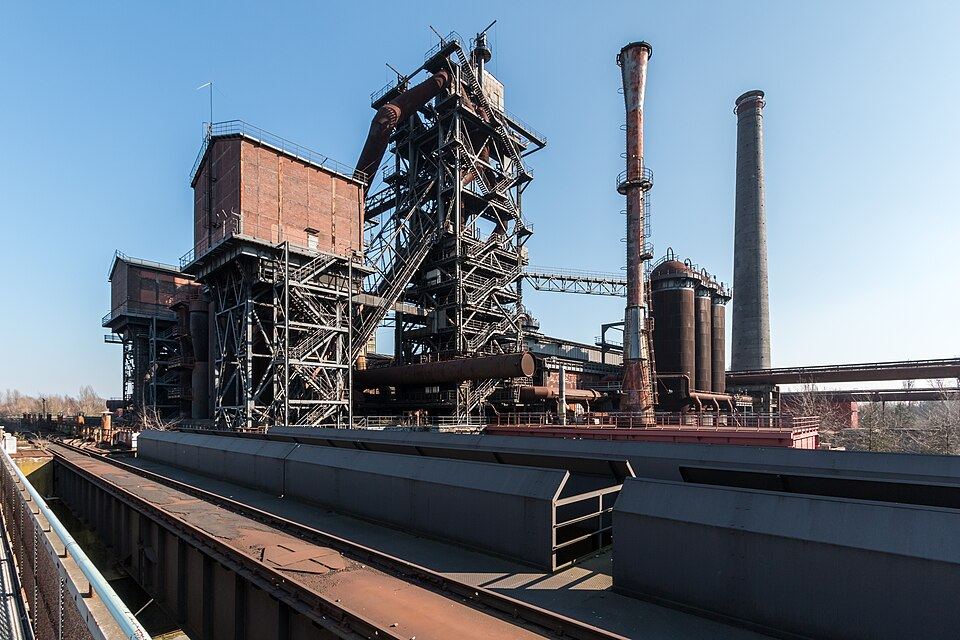
\includegraphics[width=0.6\linewidth]{images/book3/blast-furnace.jpg}

{\small Een hoogoven die als monument bewaard is (Duisburg-Nord, stilgelegd in
1985): de hoge schacht met zijn ring van leidingen voor de hete lucht, de gasafvoeren
bovenaan. (Foto: Dietmar Rabich, CC BY-SA 4.0, Wikimedia Commons.)}
\end{omfigure}

\section{Andere wegen naar een metaal}

\begin{definition}[Pyrometallurgie en hydrometallurgie]\label{def:b2:ellingham:metallurgy}
\emph{Pyrometallurgie}\index{pyrometallurgie} wint een metaal bij hoge
temperatuur, door reductie van zijn oxide in een oven. \emph{Hydrometallurgie}\index{hydrometallurgie}
wint het uit een waterige oplossing. De gebruikelijke stappen zijn
\emph{roosten}\index{roosten} (een sulfide-erts in lucht verhitten om het om te zetten in
een oxide, \ce{2ZnS + 3O2 -> 2ZnO + 2SO2}), \emph{uitlogen}\index{uitlogen}
(de verbinding van het metaal oplossen, vaak in zwavelzuur, \ce{ZnO + 2H+ ->
Zn^2+ + H2O}), zuivering van de oplossing, bijvoorbeeld door
\emph{cementatie}\index{cementatie} (reductie van de ionen van een edeler metaal
door poeder van een minder edel metaal, \ce{Cu^2+ + Zn -> Cu + Zn^2+}), en het
terugwinnen van het metaal, vaak door elektrolyse.
\end{definition}

Het diagram verklaart de taakverdeling. IJzer, zink, lood en tin worden met
koolstof in een oven gewonnen. Aluminium, waarvan de lijn bij elke haalbare
temperatuur ver onder die van koolstof ligt, wordt gemaakt door elektrolyse van zijn gesmolten oxide
(\cref{ch:b2:batteries-electrolysis}); magnesium door elektrolyse of door
reductie met silicium onder vacuüm, dat de magnesiumdamp verwijdert;
titaan door het oxide om te zetten in het chloride, \ce{TiO2 + 2Cl2 + C -> TiCl4 +
CO2} (\cref{exo:b2:reaction-free-energy:12}), en het chloride daarna te reduceren met
magnesium (het krollproces). Het meeste zink ter wereld wordt gemaakt door \omterm{def:b2:ellingham:metallurgy}{roosten},
\omterm{def:b2:ellingham:metallurgy}{uitlogen} en elektrolyse: de hydrometallurgische route levert een zuiverder metaal en
vermijdt het hanteren van zinkdamp.

\begin{omfigure}
\begin{tikzpicture}[font=\small, >={Stealth}, box/.style={draw, thick, rounded corners=2pt, align=center, minimum height=0.9cm, fill=white, text width=2.3cm}]
  \node[box] (r) at (0,0) {roosten\\ \ce{ZnS} $\to$ \ce{ZnO}};
  \node[box] (l) at (3.2,0) {uitlogen\\ in \ce{H2SO4}};
  \node[box] (c) at (6.4,0) {zuivering\\ (cementatie)};
  \node[box] (e) at (9.6,0) {elektrolyse\\ \ce{Zn^2+} $\to$ \ce{Zn}};
  \draw[->, thick] (r) -- (l); \draw[->, thick] (l) -- (c); \draw[->, thick] (c) -- (e);
  \draw[->, thick, black!60] (r.north) -- ++(0,0.7) node[above] {\ce{SO2} $\to$ zwavelzuur};
  \draw[->, thick, omThm] (e.south) -- ++(0,-0.6) -| (l.south) node[pos=0.25, below] {zuur teruggevoerd};
  \draw[->, thick] (e.east) -- ++(0.8,0) node[right] {zink};
\end{tikzpicture}

{\small De hydrometallurgische route naar zink. Het zwaveldioxide van de rooster
wordt omgezet in het zwavelzuur voor het \omterm{def:b2:ellingham:metallurgy}{uitlogen}; het zuur dat aan de
anode van de elektrolyse geregenereerd wordt, gaat daarheen terug.}
\end{omfigure}

\section{Oefeningen}

\begin{exercise}[$\star$]\label{exo:b2:ellingham:1}
Schrijf de reacties op die voorgesteld worden door de lijnen van koper(I)oxide, aluminiumoxide, koolstofmonoxide
en koolstofdioxide, telkens voor één mol \ce{O2}.
\end{exercise}

\begin{exercise}[$\star$]\label{exo:b2:ellingham:2}
Schrijf met de CODATA-sleutelwaarden ($\Delta_f H^\circ(\ce{ZnO}) = \qty{-350.46}{kJ/mol}$,
$S^\circ$: \ce{ZnO} 43.65, \ce{Zn} 41.63, \ce{O2} \qty{205.15}{J/(K.mol)})
$\Delta_r G^\circ(T)$ op van \ce{2Zn + O2 -> 2ZnO} voor vast zink.
\end{exercise}

\begin{exercise}[$\star$]\label{exo:b2:ellingham:3}
Som aan de hand van het diagram de metalen op die chroom(III)oxide kunnen reduceren bij
\qty{1500}{K}, en die welke dat niet kunnen.
\end{exercise}

\begin{exercise}[$\star$]\label{exo:b2:ellingham:4}
Verklaar het teken van de helling van elk van de drie koolstoflijnen.
\end{exercise}

\begin{exercise}[$\star\star$]\label{exo:b2:ellingham:5}
Bereken de \omterm{def:b2:ellingham:oxygen-pressure}{evenwichtszuurstofdruk} van kwik(II)oxide bij \qty{600}{K}
(kwik vloeibaar, $\Delta_r H^\circ = \qty{-181.6}{kJ}$, $\Delta_r S^\circ =
\qty{-216.5}{J/K}$ per mol \ce{O2}). Wordt kwik bij die temperatuur in lucht geoxideerd?
\end{exercise}

\begin{exercise}[$\star\star$]\label{exo:b2:ellingham:6}
Bereken $\Delta_r G^\circ$ bij \qty{298}{K} van de thermietreactie, \ce{Fe2O3 +
2Al -> Al2O3 + 2Fe}, gegeven $\Delta_f G^\circ = \qty{-743.5}{kJ/mol}$ voor
\ce{Fe2O3} en \qty{-1582.3}{kJ/mol} voor \ce{Al2O3}, en zeg waarom de reactie,
hoewel zeer \omterm{def:b2:reaction-free-energy:exergonic}{exergonisch}, niet bij kamertemperatuur op gang komt.
% ledger: janafG:Fe2O3.298, janafG:Al2O3.298
\end{exercise}

\begin{exercise}[$\star\star$]\label{exo:b2:ellingham:7}
Zoek in het diagram de temperatuur waarboven koolstof ijzer(II)oxide reduceert
tot ijzer met vorming van koolstofmonoxide, en schrijf de reactie op.
\end{exercise}

\begin{exercise}[$\star\star$]\label{exo:b2:ellingham:8}
Bij \qty{1100}{K} is $\Delta_f G^\circ(\ce{CO}) = \qty{-209.1}{kJ/mol}$ en
$\Delta_f G^\circ(\ce{CO2}) = \qty{-396.0}{kJ/mol}$. Bereken $K^\circ$ van het
\omterm{def:b2:ellingham:boudouard}{boudouardevenwicht} en de molfractie koolstofmonoxide boven koolstof bij
\qty{1}{bar}. Wat gebeurt er met het gas, in contact met roet of ijzer, wanneer het
tot \qty{700}{K} wordt afgekoeld?
% ledger: janafG:CO.1100, janafG:CO2.1100
\end{exercise}

\begin{exercise}[$\star\star$]\label{exo:b2:ellingham:9}
Waterstof wordt soms gebruikt om wolfraamoxide te reduceren. Leg met de lijn van water
uit waarom waterstof bij hoge temperatuur een betere reductor is dan koolstofmonoxide,
maar bij lage temperatuur een slechtere.
\end{exercise}

\begin{exercise}[$\star\star\star$]\label{exo:b2:ellingham:10}
Magnesiumoxide kan door silicium gereduceerd worden, \ce{2MgO + Si -> SiO2 + 2Mg}, hoewel
de lijn van siliciumdioxide bij elke temperatuur van het diagram boven die van magnesiumoxide ligt.
Bij \qty{1500}{K} is magnesium een gas en geven de tabellen, per mol
\ce{O2}, \qty{-845.5}{kJ} voor magnesiumoxide en \qty{-643.7}{kJ} voor siliciumdioxide.
Bereken $\Delta_r G^\circ$ van de reductie, en daarna de druk van de magnesiumdamp
waaronder ze voorwaarts verloopt. Hoe benut een vacuümoven dit?
% ledger: janafG:MgO.1500, janafG:SiO2.1500
\end{exercise}

\begin{exercise}[$\star\star\star$]\label{exo:b2:ellingham:11}
Bereken de \omterm{def:b2:equilibrium-shifts:variance}{variantie} van het systeem \ce{FeO(s)}, \ce{Fe(s)}, \ce{CO(g)},
\ce{CO2(g)} in evenwicht. Wat betekent dat voor het gas dat het bovenste deel
van een hoogoven verlaat?
\end{exercise}

\begin{exercise}[$\star\star\star$]\label{exo:b2:ellingham:12}
Koper wordt uit zijn uitloogoplossing gezuiverd door \omterm{def:b2:ellingham:metallurgy}{cementatie} met ijzerschroot.
Bereken met de standaardpotentialen van het deel van jaar~1 ($E^\circ(\ce{Cu^2+}/\ce{Cu})
= \qty{0.34}{V}$, $E^\circ(\ce{Fe^2+}/\ce{Fe}) = \qty{-0.41}{V}$) de
evenwichtsconstante van \ce{Cu^2+ + Fe -> Cu + Fe^2+} en de resterende
concentratie koperionen wanneer de oplossing \qty{1.0}{mol/L}
\ce{Fe^2+} bevat.
\end{exercise}

\section{Probleem: zink uit het vuur}

\begin{problem}[{Weekendprobleem --- de ellinghamlijnen van zinkoxide en van
koolstofmonoxide, de temperatuur waarbij koolstof zinkoxide reduceert, de
variantie van de oven, en de condensatie van zinkdamp}]
\label{pb:b2:ellingham:1}
Vóór de elektrolyse werd zink gemaakt door zijn oxide met koolstof te verhitten in
retorten van klei. Gegevens (CODATA, en de JANAF-tabel van zink): $\Delta_f H^\circ(\ce{ZnO})
= \qty{-350.46}{kJ/mol}$; $S^\circ$ (\unit{J/(K.mol)}): \ce{ZnO} 43.65, \ce{Zn}
41.63, \ce{O2} 205.15; zink smelt bij \qty{692.7}{K} ($\Delta_{\text{fus}}H =
\qty{7.32}{kJ/mol}$) en kookt bij \qty{1180.2}{K} onder \qty{1}{bar}
($\Delta_{\text{vap}}H = \qty{115.3}{kJ/mol}$). Voor \ce{2C + O2 -> 2CO} geven de
tabellen $\Delta_r G^\circ = \qty{-418.2}{kJ}$ bij \qty{1100}{K} en
\qty{-453.0}{kJ} bij \qty{1300}{K}.
% ledger: dfh:ZnO_cr, s0:ZnO_cr, s0:Zn_cr, s0:O2_g, hT:Zn_cr.692, hT:Zn_l.692, hT:Zn_l.1180, hT:Zn_g.1180, dfh:Zn_g, janafG:CO.1100, janafG:CO.1300

\medskip
\noindent\textbf{Deel I --- De lijn van zinkoxide.}
\begin{enumerate}
  \item Bereken $\Delta_r H^\circ$ en $\Delta_r S^\circ$ van \ce{2Zn(s) + O2 ->
        2ZnO} bij \qty{298}{K}.
  \item Schrijf $\Delta_r G^\circ(T)$ op onder het smeltpunt.
  \item Bereken de smelt- en de verdampingsentropie van zink.
  \item Schrijf $\Delta_r G^\circ(T)$ op tussen het smelt- en het kookpunt.
  \item Schrijf haar op boven het kookpunt.
  \item Bereken de drie hellingen en leg uit waarom de laatste veel steiler is.
  \item Controleer dat de drie uitdrukkingen overeenstemmen bij de overgangstemperaturen.
\end{enumerate}

\medskip
\noindent\textbf{Deel II --- De koolstoflijn.}
\begin{enumerate}[resume]
  \item Schrijf uit de twee getabelleerde waarden de lijn van \ce{2C + O2 -> 2CO} in
        de vorm $a + bT$ tussen \qty{1100}{K} en \qty{1300}{K}.
  \item Leid haar $\Delta_r S^\circ$ af en verklaar het teken.
  \item Schrijf de reductie \ce{ZnO + C -> Zn(g) + CO} op en haar $\Delta_r
        G^\circ(T)$ als verschil van de twee lijnen (per mol \ce{O2}).
  \item Zoek de temperatuur waarbij de twee lijnen elkaar snijden.
  \item Waarom is het belangrijk dat deze temperatuur boven het kookpunt
        van zink ligt?
\end{enumerate}

\medskip
\noindent\textbf{Deel III --- De retort.}
\begin{enumerate}[resume]
  \item Bereken de \omterm{def:b2:equilibrium-shifts:variance}{variantie} van het systeem \ce{ZnO(s)}, \ce{C(s)}, \ce{Zn(g)},
        \ce{CO(g)}, waarbij zink en koolstofmonoxide alleen door de reductie gevormd worden.
  \item Wat zijn in een retort bij \qty{1300}{K} onder \qty{1}{bar} de partiële
        drukken van zink en koolstofmonoxide als de reactie volledig is?
  \item Bereken $\Delta_r G^\circ$ van de reductie bij \qty{1300}{K} en de
        bijbehorende $K^\circ$.
  \item Leg uit waarom de retort iets boven de snijtemperatuur gebruikt wordt
        en niet ver erboven.
\end{enumerate}

\medskip
\noindent\textbf{Deel IV --- De condensor.}
\begin{enumerate}[resume]
  \item De damp wordt naar een koelere condensor geleid. Schrijf de reactie op waarmee
        zinkdamp door koolstofdioxide opnieuw geoxideerd kan worden.
  \item Leg met het diagram uit waarom het gas vrij van koolstofdioxide moet
        blijven.
  \item Waarom moet het zink snel en niet langzaam gecondenseerd worden?
  \item Bereken de massa koolstof die per ton zink nodig is, met de
        reductie zoals geschreven.
  \item Bereken de warmte die de reductie bij ongeveer \qty{1300}{K} per ton zink
        opneemt (neem $\Delta_r H^\circ$ uit de uitdrukkingen van Deel I
        en II).
  \item Geef de temperatuur waarboven koolstof onder standaardomstandigheden
        zinkoxide reduceert.
\end{enumerate}
\end{problem}
